\section{Hazard Analysis and Critical Control Point (HACCP) Plan}
% Specific focus on the safety of the system's processes and food outputs

% HACCP is a systematic approach to the identification, evaluation, and control of food safety hazards. A HACCP Plan is the written document which is based upon the principles of HACCP and which delineates the procedures to be followed.
% The Teams’ HACCP Plan should follow the principles and guidelines of a HACCP Plan as described by the U.S. National Advisory Committee on Microbiological Criteria for Foods (NACMCF) and the associated prerequisite programs (where applicable).
% The Basic HACCP Plan desired at this Progress Report stage (May 31 deadline) is only expected to be a starting point for the final Basic HACCP Plan expected to be a part of the final report (due in January 2023).

% Def'n of terms: https://www.fda.gov/food/hazard-analysis-critical-control-point-haccp/haccp-principles-application-guidelines#princ
% HACCP reference: https://spinoff.nasa.gov/moon-landing-food-safety?utm_source=TWITTER&utm_medium=KathyLueders&utm_campaign=NASASocial&linkId=141839394

\subsection{Food Production System Description}
% Incl. flowchart

PeaPod uses automated control systems to generate desired environments. These are air thermoregulation, humidity control, LED lighting, and an aeroponics system. They are automated by an onboard computer and housed in a "control module" at the top of the unit. This lets power be "multiplied" for extended PeaPods by adding more control modules in a controller-follower topology.

PeaPod is an automated plant growth environment, comprised of several control systems regulated by an automation and monitoring system within a modular, cubic housing. It can generate any desired environment while collecting data on plant growth and improving yields. Due to the wide range of actuation for each control system's environment parameter, and the extendable housing topology, the growth environment is adaptable to any plant or mission requirements. In addition, plant growth support platforms (with watering system) and lighting systems are built on modular "trays" mounted to the inside of the housing so the user can position plants and lights to accommodate any plant size.

PeaPod's control systems are made of environmental controls (feedback loops with sensors) and plant inputs (set-states):
\begin{itemize}
    \item\textit{Lighting}: LEDs, from near-ultraviolet to near-infrared. Dimmable drivers for precision spectrum and intensity control. Efficient, precise emission spectrum, low heat.
    \item \textit{Aeroponics}: Reverse osmosis (RO) water is pressurized by a pump (with sensor for safety cutoff), brought to temperature, nutrient-dosed and pH-balanced by custom peristaltic pumps (allows for accurate dosing, and prevents backflow under pressure), and forced through nozzles to generate mist. Root zone air temperature is regulated in the same way as the leaf zone system. Exceptions include an aluminum water block (vs internal heat sink and fan) and a single temperature sensor after the block for PID feedback in a flowing system. Runoff water is recycled. Water-efficient (98\% less water use than farming), nutrient-efficient (60\% less use than farming), no pH/nutrient "feedback" loop or waste water (common in hydroponics), increased root oxygenation.
    \item \textit{Leaf-Zone Thermoregulation}: Leaf zone air temperature is regulated by a thermoelectric heat pump. Fans blow air over heat sinks connected to either face of a Peltier tile to circulate air and dissipate heat. A Proportionate-Integral-Derivative (PID) control system is informed by temperature sensors, and controls the direction and magnitude of the heat transfer. Low complexity, high safety/reliability, easy to automate (bidirectional, precisely dimmable, PID tuning).
    \item \textit{Humidity Regulation}: Leaf zone humidity is regulated by a dead-zone bang-bang control system informed by humidity sensors.
    \begin{itemize}
        \item \textit{Humidification}: RO water is supplied to a tank with a fine mesh piezoelectric disc. A controllable driver circuit oscillates the disk, producing water vapour. Easy to automate.
        \item \textit{Dehumidification}: A dry silica gel bead cartridge is covered by servo-actuated "shutters" to control dehumidification. Fans draw humid air through a HEPA filter into the desiccant and back into the growth environment on demand. The beads change color to indicate water saturation. The crew is then notified to swap and "recharge" via evaporation in a standard oven.
    \end{itemize}
    \item \textit{Gas Composition Regulation and Exchange}: Oxygen and carbon dioxide levels are managed by gas exchange. Input and output ports allow fans to draw air into and out of the system. HEPA filters remove microbes and aerosols, and servo-actuated "shutters" prevent unintended exchange. Gas concentration sensors inform a bang-bang control system for port activation.
\end{itemize}

\begin{figure}[h!]
  \centering
  \frame{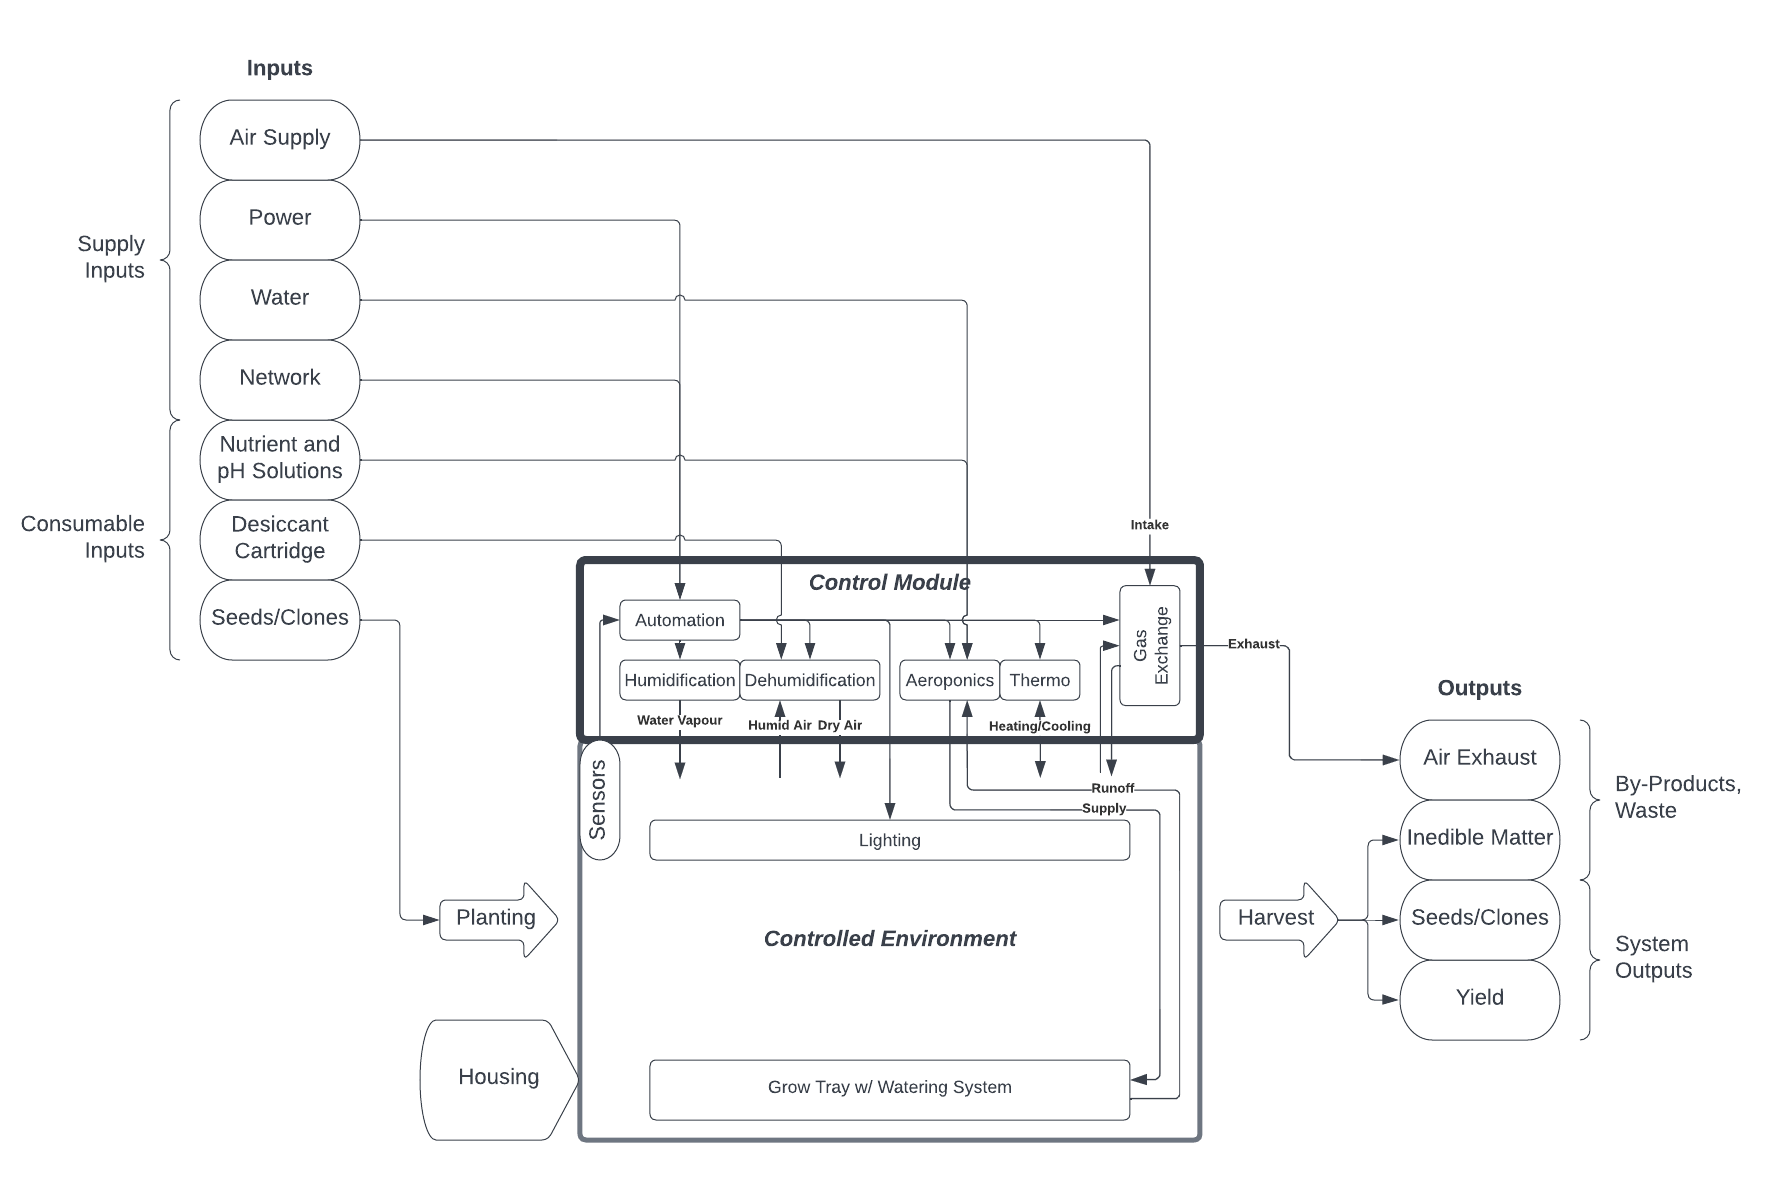
\includegraphics[width=\textwidth]{../assets/figures/system.png}}
  \caption{System overview.}
  \label{fig:system}
\end{figure}

\clearpage

\subsection{Critical Points}
%assembly: only approved parts that have been checked for leaks, contamination, materials, air-tightness

%seeds: vetted and tested breed from an approved supplier, not opened until moment of planting, food safety steps followed while doing so (hand washing, gloves, masks, hairnet...)

%growth medium: tested for bacteria/pests, handled carefully before installation

%system inputs: filtered air, clean water, properly sourced nutrients, all tested by appropriate standards

%maintenance: plants properly isolated when non-food safe materials are present---i.e. if LED boards need to be swapped, if something needs to be greased, if something needs to be glued

%harvesting: all food safety guidelines to be followed - hand washing, gloves, masks, washing, etc.

%re-planting: checking for no old growth medium, sanitizing growth tray with food-safe sanitizer

\subsubsection{Critical Point A}
% Repeat for all control points

\textbf{Hazard Description}
% aka hazard analysis, discover CCPs

\textbf{Critical Limits}
% What is the safe range AND the failure conditions for the CCP

\textbf{Monitoring Procedures}
% How do we know the state of the CCP

\textbf{Deviation Procedures}
% aka corrective actions
% How do we keep the CCP within range?

\textbf{Associated Documents}
% record-keeping and documentation procedures

% TODO: Verification Procedures?

\subsection{Standard Test Record}
% TODO: What exactly is this?

\subsubsection{Purpose and Summary}

\subsubsection{Safety and Quality}

\subsubsection{Test Processes}

\textbf{Preparation of Inputs}\\


\textbf{Verification}\\


\textbf{Setup, Maintenance, and Collection Protocols}\\


\textbf{Storage}\\


\textbf{Cleanup and Turnover}\\


\subsubsection{Closeout}

